\documentclass[review]{elsarticle}
\usepackage{lineno,hyperref}
\usepackage{subcaption}
\usepackage{siunitx}
\usepackage{booktabs}
\usepackage{graphicx}
\usepackage{appendix}
\usepackage{amsmath} 
\usepackage[hang,flushmargin]{footmisc} 
\usepackage{xcolor}
\usepackage{float}
\usepackage{array,multirow}
\usepackage{hyperref}
\usepackage{setspace}
\usepackage{stmaryrd}
\usepackage{enumitem}
\usepackage{rotating}
\usepackage{adjustbox}
\usepackage{array}
\usepackage{booktabs}
\usepackage{xcolor,colortbl}
\usepackage{amsmath} 
\usepackage{amsfonts} 
\usepackage{amssymb}
\usepackage{makecell}
\usepackage{amsmath}
\usepackage{nicefrac}
\usepackage{todonotes}
\usepackage{multirow}
\modulolinenumbers[1]
\usepackage{lineno}
\usepackage{xcolor}
\usepackage{pifont}
\renewcommand\theadfont{\normalsize}


\usepackage[final]{changes}
% \usepackage[markup=underlined]{changes}
\usepackage[ruled,vlined,linesnumbered,lined,boxed,commentsnumbered]{algorithm2e}
\newcommand\mycommfont[1]{\footnotesize\ttfamily\textcolor{blue}{#1}}
\SetCommentSty{mycommfont}
\newcommand{\BREAK}{\STATE \algorithmicbreak}
\modulolinenumbers[1]
\setlength{\parindent}{0em}
\journal{Sustainable Energy, Grids and Networks}
\bibliographystyle{elsarticle-num}

\begin{document}
\begin{frontmatter}

\title{Downscaling European decarbonization scenarios of the heating sector to the Austrian community level: Assessing the heat density gap of centralized heat networks between 2050 and today}
\author[1,2]{Sebastian Zwickl-Bernhard\corref{cor1}}
\ead{zwickl@eeg.tuwien.ac.at}
\author[2]{Daniel Huppmann}
\author[1]{Antonia Golab}
\author[1]{Hans Auer}
\cortext[cor1]{Corresponding author}
\address[1]{Energy Economics Group (EEG), Technische Universität Wien, Gusshausstrasse 25-29/E370-3, 1040 Wien, Austria}
\address[2]{Energy, Climate and Environment (ECE) Program,  International Institute for Applied Systems Analysis (IIASA), Laxenburg, Austria}

\begin{abstract}
	The core objective of this work is to downscale European deep decarbonization scenarios of the heating sector to the Austrian community level in 2050 to obtain an estimation of future demand for different heating technologies on smaller geographical scale. We use tailor-made downscaling techniques accounting for infrastructure needs of heat sources, the network topology of centralized heat networks, and population density. The results show that centralized heat networks play an important role in the highly efficient heat supply of densely populated areas in 2050. However, the projected heat density of supply areas is significantly lower than today despite high connection rates (in average greater than \SI{85}{\%}). We identify a heat density gap of at least \SI{7.42}{\frac{GWh}{km^2}} considering \SI{10}{\frac{GWh}{km^2}} as today's minimum required value. We conclude that future yes/no decisions of centralized heat networks should take enhanced account of the highly efficient use of sustainable and local heat sources in addition to the achievable heat density. Policy-makers should incorporate the development of lower heat densities resulting from decarbonization measures in the benchmarking of centralized heat networks efficiency.  
\end{abstract}

\begin{keyword}
	Downscaling, Centralized heat networks, Heat density, Network topology, Infrastructure requirements
\end{keyword}
\end{frontmatter}

\linenumbers
\section{Introduction}
To implement the pathway in line with the Paris Climate Agreement \cite{agreement2015paris} as analy\replaced{z}{s}ed by the IPCC's \emph{Special Report on Global Warming of 1.5°C} (SR15) \cite{book}, the European Commission has set deep decarbonization targets together with national governments. In particular, the \replaced{\textit{EU Green Deal}}{"EU Green Deal"} describes the concrete goals in Europe, namely, a climate-neutral and resource-conserving economy and society \deleted{(see, e.g., }\cite{kemfert2019green}\deleted{)}. The overarching goal is to reduce carbon emissions to net-zero and hence achieve climate neutrality by 2050. The principles of a net-zero, decarbonized society are based on three key points: (i) reduction of the energy demand \deleted{(see, e.g., Oshiro et al. \cite{oshiro2021enabling} and Grubler et al. }\cite{grubler2018low}\deleted{)}, (ii) deployment and generation of renewable energy technologies \deleted{(see, e.g., Bakhtavar et al. }\cite{bakhtavar2020assessment}\deleted{)}, and (iii) an increase in efficiency regarding the provision of energy services and the associated optimal utilization of sustainable energy sources.\vspace{0.3cm}

To achieve these long-term ambitions, the European Commission recently presented \replaced{\textit{Fit for 55}}{"Fit for 55"}, a \deleted{concrete} roadmap \added{with specific actions and targets} \replaced{until}{to} 2030. This program commits to a \SI{55}{\%} reduction in CO\textsubscript{2} emissions in 2030 compared to \deleted{to} those in 1990 \cite{european_commission_european_2019}. The concrete measures affect almost all sectors of the energy system and should lead to a significant efficiency improvement and a massive overall reduction in fossil fuels. It implies, among others, binding annual targets to reduce energy consumption and to extend the already established EU emissions trading system (EU ETS) to new sectors. In addition to transportation, the building sector will be part of the EU ETS in the future. In the building sector, using the annual anchored emissions reduction, this means a defined roadmap to complete decarbonization of the heating and cooling demand. In this paper, we look at what deep decarbonization of building heating demand may look like in 2050 in Austria and the implications of the corresponding sustainable energy mix for \replaced{district heating}{centralized heating networks}.

\subsection{Implications of decarbonization on the heating sector}
The scope of changes required by 2030/2050 in the heating sector becomes even clearer at the national level. In Europe, the \deleted{average }share of renewable energies in the heating and cooling sector in 2018 is only just above \SI{20}{\%} on average\deleted{, for all EU member states} \cite{eurostat_reference}. \added{In Austria, it reaches 34\%}\deleted{It is, in fact, higher in some countries, for example, in Austria, it is above 34\%}. However, fossil fuels continue to dominate there as well. \added{In 2015, the heat demand for low-temperature heat services in Austria was approximately} \SI{96}{TWh}\added{ \cite{burandt2018genesys}. Thereby, natural gas, oil and coal account for almost 45\% of space heating and hot water demand in the residential building sector \cite{oesterreichsenergie}. The share of district heating reaches almost 15\% and more than \replaced{one million}{1,100,000} households are connected to district heating networks.}\footnote{\added{See }\ref{appendixC} \added{for a detailed overview of the Austrian heat market as well as references \cite{oesterreichsenergie} and \cite{buchele2015bewertung} for more details.}}.\deleted{To be even more specific for the heating sector, o}\added{Nevertheless, o}f the nearly 4,000,000 residential dwellings in Austria, more than \replaced{one million}{900,000} are heated with natural gas, and more than 500,000 with oil \cite{statistik_austria}. If these heating systems are converted to renewable energy supply by 2050, this corresponds to a retrofitting of 50,000 units per year, or more than 130 per day - only in Austria. To achieve this goal, measures that go beyond the electrification of heat supply are necessary, which may requre an expansion of district heating networks. This holds true even when substantial heat saving measures are installed such as better insulation of buildings \cite{jalil2018spatially}.\vspace{0.3cm}

\replaced{District heating is}{Centralized heating networks are} particularly advantageous for supplying densely populated or urban areas because of high heat densities \cite{inage2020development}. \added{Particularly in Europe, there are good conditions for district heating \cite{persson2019heat}.} In addition to heat density, the connection rate is a key factor determining the efficiency of district heating/cooling networks and thus their implementation. In Austria, a benchmark of \SI{10}{GWh \per km^2} at a connection rate of \SI{90}{\%} is currently used when deciding whether to supply an area with district heating\footnote{\url{http://www.austrian-heatmap.gv.at/ergebnisse/}}. This reference value is in line with findings regarding district heating networks also from the Scandinavian region (Denmark, Sweden, and Finland) \cite{zinko2008district}. These are rough estimates, but they do allow an initial assessment of the economic viability or feasibility of a district heating network. In a detailed consideration and evaluation of district heating networks, numerous factors play a decisive role. \added{For example, the design and topology of district heating networks has a significant impact on their cost-effectivness \cite{nussbaumer2016influence}.}\deleted{Nussbaumer and Thalmann \cite{nussbaumer2016influence} thoroughly elaborate on the network design and its impact on the profitability of centralized heat networks.} \added{In addition, the cost-optimized heat supply is also influenced by the location of heat generation units/sources within the networks \cite{laasasenaho2019gis}.} \deleted{In their study, Laasasenaho et al. \cite{laasasenaho2019gis} emphasize the optimal location of heat generation units/sources within centralized heat networks, enabling a cost-optimized heat supply.} \deleted{Gopalakrishnan and Kosanovic \cite{gopalakrishnan2014economic} focus on the optimal heat generation technology dispatch.} When examining the economic viability of district heating networks, building renovation measures must also be taken into account \deleted{(see, e.g., }\cite{andric2018impact}\deleted{ and \cite{rabani2021achieving})}. \replaced{A recent study shows}{Hietaharju et al. \cite{hietaharju2021stochastic} recently show in their analysis} that a $2-3$\SI{}{\%} building renovation rate per year results in a $19-28$\SI{}{\%} decrease of the long-term district heating demand \added{\cite{hietaharju2021stochastic} which consequently also reduces the heat densities of networks.}. \deleted{This also reduces the heat density.} However, studies show that a reduction in heat density is not necessarily a barrier to district heating networks \cite{persson2011heat}. \added{For example, energy taxes which can certainly be expected in the future (e.g., higher taxes on fossil fuels) can improve the profitability of sparse district heating networks \cite{reidhav2008profitability}.}\deleted{Reidhav and Werner \cite{reidhav2008profitability} show how energy taxes can improve the profitability of sparse district heating networks in Sweden.} Following these considerations and in light of ambitious CO\textsubscript{2} reduction targets, it can also be assumed that the rising CO\textsubscript{2} price can have an effect similar to the energy tax. \replaced{Naturally}{Of course}, this is valid only in the case of deep decarbonization of the generation mix feeding into \replaced{district}{centralized} heat\added{ing} networks. \added{In general, there are a variety of alternatives to decarbonize the energy mix of district heating networks. Among others, geothermal \cite{kyriakis2016towards}, biomass \cite{di2014low}, waste \cite{hiltunen2020highly} and heat recovery from industrial excess heat \cite{buhler2017industrial} are likely to be the primary heat sources in sustainable district heating networks.}\deleted{Di Lucia and Ericsson \cite{di2014low} show that biomass significantly contributed to the decarbonization of the district heating network and replaced fossil fuels in the feed-in generation mix in Sweden. In their multi-criteria study, Ghafghazi et al. \cite{ghafghazi2010multicriteria} also identify wood pellets as the optimal system option for fueling district heating networks.} Eventually, the increasing cooling demand and the co-design of \replaced{district}{centralized networks for} heating and cooling \added{networks} can also increase the economic viability of these and counteract the reduction of heat density from an economic point of view \cite{zhang2021economic}.

\subsection{Implications of large-scale numerical model results at the local level}
For quantifiying solutions of complex planning problems, researchers use numerical models. In general, these models strike a balance between complexity and aggregation. Integrated assessment models (IAMs) are large numerical models covering complex interrelationships between climate, society, economics, policy, and technology \cite{dowlatabadi1995integrated}. \added{Particularly, IAM contribute to the understanding of global energy decarbonization pathways \cite{wilkerson2015comparison}}.\deleted{Wilkerson et al. \cite{wilkerson2015comparison} and van Vuuren et al. \cite{van2016carbon} deal with IAMs and their role in understanding global energy decarbonization pathways.} \replaced{Evaluating and discussing IAM involves}{Schwanitz \cite{schwanitz2013evaluating} evaluates IAMs of global climate change and discusses}, among others, the appropriate level of regional (spatial) aggregation of countries in the modeling analysis \added{\cite{schwanitz2013evaluating}}. Generalizing this aspect reveals an aspect already known but essential in the context of large numerical models. It becomes necessary for modelers to set priorities regarding the level of detail, which inevitably creates trade-offs in the analysis regarding the granularity of temporal, spatial, and other dimensions \cite{gargiulo2013long}. \added{Accordingly, }\deleted{Gambhir et al. \cite{gambhir2019review} also highlight this aspect of aggregation bias in their critical review of IAMs. They propose, among others, that }IAMs should \deleted{be} increasingly be supplemented with other models and analytical approaches \added{\cite{gambhir2019review}}. Not least for this reason, large-scale detailed energy systems models also play a significant role in the analysis of energy systems in the context of climate change. Compared to IAMs, they more strongly emphasize the level of detail in terms of techno-economic characteristics. However, the lack of granularity remains: these global systems models consider only a highly aggregated spatial resolution. To name just two selected approaches, \deleted{Capros et al. \cite{capros2012model} (}PRIMES\deleted{)} \added{\cite{capros2012model}} and \deleted{Löffler et al. \cite{loffler2017designing} (}GENeSYS-MOD\deleted{)} \added{\cite{loffler2017designing}} \replaced{are}{provide} energy system models focusing on the European energy system with a spatial resolution at the country level. Further approaches are needed to disaggregate results obtained at the country level to finer scales, such as districts, neighborhoods, and other local levels. In this context, \deleted{Backe et al. \cite{backe2021heat} provided }a novel approach in the context of merging local activities/behavior in sustainable local communities into a large energy system model (bottom-up linkage) \added{is presented in \cite{backe2021heat}}. In \replaced{this}{their} study, \deleted{they integrated }local flexibility options \added{are integrated} into the global energy system model EMPIRE, which provides, in principle, only country-level resolution. This and other work confirms the emerging trend of making top-down and bottom-up linkages between different spatial-temporal levels of resolution to drive decarbonization across all sectors.\vspace{0.3cm}

\subsection{Objective and contribution of this work}
Against this background, the core objective of this work is downscaling European decarbonization scenarios of the heating sector to the community \replaced{or}{/} distribution grid level serving end-users in 2050. In particular, downscaling considers the highly efficient and local use of sustainable heat sources in \replaced{district}{centralized} heat\added{ing} networks (e.g., \added{geothermal sources, }co-firing \added{synthetic gas and }hydrogen in cogeneration plants and large-scale waste utilization\deleted{, etc.}). In addition, the topography of district heating networks is of particular importance and plays a crucial role in applied downscaling. This allows estimates of realistic \deleted{and cost-effective} decarbonized district heating networks in 2050 to be obtained, which can be compared with existing networks. Thereby, the heat density of district heating networks serves as a comparative indicator and permits a rough estimation of the changes needed for \replaced{district}{centralized} heating networks considering the 1.5°C climate target. An Austrian case study is conducted, downscaling the \added{cost-effective} results of the heating sector in 2050 from the large numerical energy system model GENeSYS-MOD, from the country to the community\replaced{or}{/} distribution grid levels.\vspace{0.3cm}

The method applied \added{(section \ref{methodology})} consists of three different scenario-independent downscaling techniques. In the first technique, proportional downscaling uses population as a stylized proxy (section \ref{pop}). In the second, a sequential downscaling approach is presented, disaggregating from the country level to the sub-region level. Thereby, the population density and infrastructure requirements of heat \added{sources/generation }technologies serve as additional criteria in the downscaling (section \ref{alg1}). Finally, an iterative downscaling algorithm is presented. The algorithm applies benchmarking based on graph-theory. It computes \replaced{district heating}{centralized heat supply} at the local (community) level, see section \ref{alg2}. Section \ref{results} presents and discusses the results of this work. Section\deleted{s \ref{res:1} and} \ref{res:2} show\added{s} heat generation by source at different spatial levels. Sections \ref{res:3} and \ref{res:4} present \replaced{district heating networks}{centralized heat networks} at a high spatial granularity. Section \ref{res:5} synthesizes the results of \replaced{district}{centralized} heat\added{ing} networks and compares heat densities of \replaced{district heating}{centralized heat networks} in 2050 with today's values. \added{Section \ref{sens:hp} presents a sensitivity analysis of the heat density of district heating regarding the allocation of heat generation by heat pumps feeding into district heating networks. }Section \ref{conclusions} concludes this work and provides an outlook for future work.
\newpage
\section{Materials and methods}\label{methodology}
This section explains the methodology developed in this work. First, Section \ref{pop} describes the proportional spatial downscaling using population as a proxy. This downscaling technique is a well-established approach for disaggregation and is often used in scientific and practical studies. Building upon, Section \ref{alg1} presents the sequential downscaling and Section \ref{alg2} the iterative downscaling algorithm in detail. Finally, Section \ref{open} concludes this section and explains the open-source tools used in this work.

\subsection{Proportional spatial downscaling using population as a proxy}\label{pop}
Proportional downscaling is a well-established technique and is commonly used. Equation \ref{eq:1} shows the primary expression of proportional downscaling, exemplarily, for the disaggregation of the energy demand $d$ from the country to the local level, using population $p$ as a proxy.  
\begin{align}\label{eq:1}
d_{local}=\frac{p_{local}}{p_{country}} \cdot d_{country}
\end{align}
The fields of application are not limited to the modeling of energy systems. Moreover, it is applied in different fields of scientific and practical studies. The reason for this is the intuitive application and that it offers possibilities for tailor-made adaptions, in particular, related to the downscaling driver and proxy \cite{van2006downscaling}. In this context, van Vuuren et al. \cite{van2006downscaling} provide a comprehensive analysis of different proxies for the downscaling of global environmental change, including, among others, gross domestic product (GDP) and emissions as a proxy. However, in the context of downscaling aggregated values of energy systems, one often finds proportional downscaling using population as a proxy (see, e.g., Ahn et al. \cite{ahn2019downscaled}, van Vuuren et al. \cite{van2010downscaling}, and Alam et al. \cite{alam2018downscaling}). For further information, we refer the reader here to the study in \cite{van2010downscaling}, providing a systematic classification of downscaling techniques going far beyond the simple proportional downscaling method discussed so far. The reader can find population-based downscaling in their categorization under algorithmic and proportional downscaling. In addition, they showed that novel downscaling methods have emerged in recent years as the scientific community has increasingly recognized the necessity for spatially and temporally disaggregation.

\subsection{Sequential downscaling (from the country to the sub-region level)}\label{alg1}
The sequential downscaling algorithm (Algorithm 1) is developed to downscale the heat generation by source from the country to the sub-region level. Before explaining the algorithm in detail, Table \ref{tab:nuts} provides an overview of the spatial nomenclature of this work using the European nomenclature of territorial units for statistics\footnote{\url{https://ec.europa.eu/eurostat/web/nuts/background}.} (NUTS) and gives some examples of Austria. In particular, the different spatial levels of the applied downscaling are marked in gray. According to the NUTS nomenclature, Algorithm 1 downscales from NUTS0 to the NUTS3 level.\vspace{0.3cm}

\definecolor{Gray}{gray}{0.95}
\begin{sidewaystable}
	\centering
	\setlength{\extrarowheight}{.5em}
	\scalebox{0.85}{
		\begin{tabular}{cccc}
			\toprule
			NUTS level  & Description & Number& Example (population)\\\hline
			\cellcolor{Gray}NUTS0 & \cellcolor{Gray}Country level & \cellcolor{Gray}1 & \cellcolor{Gray}AT Austria (8.86 millions)\\
			NUTS1 & Major socio-economic regions & 3 & AT3 Western Austria (2.78 millions)\\
			NUTS2 & Basic regions for the application of regional policies (federal states) & 9 & AT31 Upper Austria (1.48 millions)\\
			\cellcolor{Gray}NUTS3 & \cellcolor{Gray}(Small) sub-regions for specific diagnoses (political/court districts) & \cellcolor{Gray}35 & \cellcolor{Gray}AT312 Linz-Wels (529 thousands)\\
			\cellcolor{Gray}LAU (former NUTS4/5) & \cellcolor{Gray}Subdivision of the NUTS 3 regions (communities)& \cellcolor{Gray}2095 & \cellcolor{Gray}Enns AT312 Linz-Wels (11 thousands)\\ 
			\bottomrule
	\end{tabular}}
	\caption{Spatial nomenclature of different spatial levels using the NUTS nomenclature. Besides the number of regions per NUTS level, examples for the Austrian case study (incl. population) are given. The gray-colored rows mark the spatial levels used for downscaling in this work.}
	\label{tab:nuts}
\end{sidewaystable}

The purpose of the sequential downscaling algorithm is to provide a downscaling technique that considers the variation in efficiency of renewable heat sources and the increasingly role of biomass and waste heat sources, in particular, in densely populated areas. Hence, we claim that 

\begin{itemize}
	\item the limited amounts of hydrogen (and or "green" gas) should preferably be used in district heating networks if it is used for heat supply (similar to Gerhardt et al.  \cite{gerhardt2020hydrogen} and Zwickl-Bernhard and Auer \cite{zwickl2021demystifying}).
	\item high shares of biomass in the heating sector result in a high utilization rate of waste sources in waste incineration plants \cite{fruergaard2010energy}. These waste incineration plants feed into district heating and are therefore dependent on the infrastructure of centralized heating networks (see, exemplarily, Sahlin et al. \cite{sahlin2004effects}).
\end{itemize}

Besides, we claim that high shares of air-source heat pumps (or geothermal sources) in the heat supply can only be realized if it is used as a co-firing heat source in district heating networks. We therefore consider two main aspects, namely that geothermal sources will contribute significantly to decarbonizing the feed-in energy mix of existing district heating grids in the future (see, exemplarily in \cite{weinand2019developing}), and that provision of high shares of geothermal-based heat supply requires the distribution through district heating infrastructure \cite{dalla2020scenarios}. Besides, it is highly uncertain if small-scale geothermal units on the end-user's level are be economically viable in the future resulting due to expected high investment costs.\vspace{0.3cm}

In order to incorporate the above mentioned relevant technology-specific aspects, heat technologies/sources are downscaled according to their necessity of distribution infrastructure. Therefore, population density serves as a criterion, indicating the possibility of centralized heat networks. Table \ref{tab:require} provides a qualitative overview of the different heat generation technologies/sources and their heat network/infrastructure requirements. 

\definecolor{Gray}{gray}{0.85}
\begin{table}[h]
	\centering
	\setlength{\extrarowheight}{.5em}
	\scalebox{0.85}{
		\begin{tabular}{ccccc|l}
			\toprule
			\underline{Source} & \underline{Requirements} & Rural & Town/Mixed & Urban&\multirow{2}{*}{\vtop{\hbox{\strut Supporting}\hbox{\strut references}}}\\
			Heat technology & Heat network & Sparsely & Moderate & Dense&\\\hline 
			Biomass & Middle & &  \cellcolor{Gray}x & \cellcolor{Gray}x&\cite{vallios2009design,ericsson2016introduction, fruergaard2010energy}\\
			Direct electric & None &  x & x & x&\\
			Synthetic gas & Low & x & x & x&\\
			Hydrogen & High &  &  &  \cellcolor{Gray}x& \cite{jensen2020potential, dodds2015hydrogen, arsalis2019thermodynamic}\\
			Heat pump (air) & None &  x & x & x&\cite{yang2018using}\\
			Heat pump (ground) & High &  &  &  \cellcolor{Gray}x& \cite{kyriakis2016towards, unternahrer2017spatial, weinand2019developing}\\
			Heat storage & None &  x & x & x&\\
			\bottomrule
	\end{tabular}}
	\caption{Qualitative overview for heat generation technologies/sources and their requirments for heat network infrastructure. The prioritized preferences (gray cell color) of heat sources in sub-regions is marked by the gray color. In addition, selected references supporting this assumptions are cited.}
	\label{tab:require}
\end{table}

The sub-regions used for downscaling the corresponding heat source are marked. Note that the different types are characterized by population density. Exemplarily, direct electric heating is a heat generation technology with no significant heat network requirements. It is downscaled to all types of sub-regions. In contrast, hydrogen is a heat source with high requirements and thus prioritized preferences (marked by the gray cell color). The right column refers to selected references whose key findings are in line with this approach/assumptions. Building upon, the sequential downscaling algorithm is presented below (Algorithm 1).\vspace{0.6cm}

\scalebox{1}{
	\begin{algorithm}[H]
		\setstretch{1}
		\SetKwInOut{Input}{input}
		\SetKwInOut{Output}{output}
		\SetKwInput{kwInit}{Initialization}
		$t$: Heat generation by technology/source $(t \in T)$\;
		$r$: Sub-region (or NUTS3 region) $(r \in R)$\;
		\vspace{0.2cm}
		\Input{Heat generation by technology/source at NUTS0 level: $(q_{t})$;\newline
			Population density per region $r$ $(\rho_{r})$;\newline
			Total population per region $r$ $(p_{r})$;\newline
			Minimal network infrastructure requirements of $t$ $(\sigma_{t})$;\newline
			Available potential of heat network infrastructure at $r$ ($\pi_{r}$)\;}
		\vspace{0.2cm}
		\Output{Heat generation by technology/source on NUTS3 level $(\hat{q}_{t,r})$\;}
		\vspace{0.2cm}
		\kwInit{\\
			Sort elements $t$ in $T$ descending by $\sigma_{t}$\;
			$q^{heat}_{r} \longleftarrow \sum_{t} q_{t} \cdot \frac{p_{r}}{\sum_{r} p_{r}}$ \tcp*{Calculate heat demand at each sub-region}
			$\tilde{q}_{t} \longleftarrow q_{t}$ \tcp*{Available heat generation for each technology/source}
			$\pi_{r} \longleftarrow \rho_{r}$ \tcp*{Population density determines network potential}
			\vspace{0.2cm}}
		\SetAlgoLined
		\Begin{
			\ForEach{$t$}{
				$List=[~]$\tcp*{Collect valid sub-regions}
				$demand=0$\tcp*{Reamining demand that needs to be covered}
				$R^{'}=R\setminus \{\forall r \in R: \pi_{r} \leq \sigma_{t}\}$\tcp*{Get valid sub-regions by criteria}
				\ForEach{$r^{'} \in R^{'}$}{
					\If{$q^{heat}_{r} \ge 0$}{
						$List = List \cup r^{'}$\tcp*{Add valid sub-regions to collection} 
						$demand\mathrel{+}=q^{heat}_{r}$\tcp*{Total demand of valid sub-regions}}}
				\ForEach{$l \in List$}{
					$\hat{q}_{t,r} = \frac{q^{heat}_{r}}{demand}\cdot \tilde{q}_{t}$\tcp*{Population-based downscaling}
					$q^{heat}_{r} \mathrel{-}= \hat{q}_{t,r}$\tcp*{Reduce heat demand at $r$}
				}
			}
		}\caption{Sequential downscaling algorithm (NUTS0 to NUTS3)}
		\label{Alg:1}
\end{algorithm}}\vspace{1cm}
\newpage
The inputs are as follows: (i) heat generation by technology/source at the NUTS0 level, (ii) population as well as population density on the NUTS3 level, and (iii) empirical assumptions in terms of network infrastructure requirements per heat technology/source and potentials for heat network infrastructure (see Table \ref{tab:require}). The algorithm itself consists of three main parts: initialization, pre-calculations, and downscaling. First, the initialization of the algorithm sorts the heat generation technologies/sources in descending order in terms of network infrastructure requirements. Then the calculation starts with the first technology/source (highest requirements) (line 6). For this technology/source, all possible sub-regions are collected (line 9). Those sub-regions already fully supplied (no remaining heat demand) are filtered out (line 11). After further pre-calculation steps, the available amount of heat generation is downscaled to all valid sub-regions using population as a proxy. This procedure is repeated sequentially for each heat technology/source. The output of the sequential downscaling algorithm are heat generation by source and the amount of heat demand covered by centralized heat networks on the NUTS3 level.

\subsection{Iterative downscaling (from the sub-region to the community level)}\label{alg2}
This section explains the methodology of the iterative downscaling algorithm. We propose this downscaling technique projecting heat generation by technology/source from the sub-region (NUTS3) to the community level (LAU) (see Table \ref{tab:nuts}). This in-depth spatial resolution is imperative for realistic network infrastructure planning as stated by Zvoleff et al. \cite{zvoleff2009impact}. The underlying concept of iterative downscaling bases on graph theory and assessing network topology using benchmark indicators. 

\newpage
\scalebox{1}{
	\begin{algorithm}[H]
		\setstretch{1}
		\SetKwInOut{Input}{input}
		\SetKwInOut{Output}{output}
		\SetKwInput{kwInit}{Initialization}
		$s$: Stage of iteration $(s \in \{0, 1, *\})$\;
		$G^{s}$: Centralized heat network graph at stage $s$\;
		$N^{s}$: List of nodes at stage $s$: ($n^{s} \in N^{s}$)\;
		$L^{s}$: List of lines connecting nodes $k$ and $j$ at stage $s$: ($l^{s}_{k,j} \in L^{s}$)\;
		$Q^{s}$: Centralized heat generation at stage $s$: $(q^{s}_{n^{s}} \in Q^{s})$\;
		$\tilde{Q^{s}}$: On-site heat generation at stage $s$: $(\tilde{q}^{s}_{n^{s}} \in \tilde{Q^{s}})$\;
		$\Pi^{s}$: Benchmark indicator value at stage $s$ ($\pi^{s}_{n^{s}} \in \Pi^{s}$)\;
		\vspace{0.2cm}
		\Input{$G^{0}=\{N^{0}, L^{0}, Q^{0}, \tilde{Q^{0}\}}$\;}
		\Output{$G^{*}=\{N^{*}, L^{*}, Q^{*}, \tilde{Q^{*}\}}$\;}
		\vspace{0.2cm}
		\kwInit{\\
			$s=0$, $iter=True$\;	
		}
		\SetAlgoLined
		\Begin{
			\While{$iter=True$}{
				\ForEach{$n \in N\textsuperscript{s}$}{
					$\Pi^{s}_{n^{s}}=f(N^{s}, L^{s}, Q^{s})$\tcp*{Calculate benchmark indicator value}}
				$i$ with $\pi^{s}_{i}=min(\Pi^{s}$)\tcp*{Get node with lowest indicator value}
				$N^{s+1}=N^{s} \setminus i$\tcp*{Remove node from graph obtaining next stage}
				$\tilde{q} = \sum_{N^{s+1}} \tilde{q}^{s}_{n^{s}}$\tcp*{Calculate available on-site heat generation}
				\eIf{$\tilde{q} \geq q^{s}_{i}$}{
					\ForEach{$n^{s+1}$}{
						$q^{s+1}_{n^{s+1}} = q^{s}_{n^{s}}+\frac{q^{s}_{i}}{\tilde{q}}\cdot \tilde{q}^{s}_{n^{s}}$\tcp*{Increase centralized heat amount}
						$\tilde{q}^{s+1}_{n^{s+1}} = \tilde{q}^{s}_{n^{s}}-\frac{q^{s}_{i}}{\tilde{q}} \cdot \tilde{q}^{s}_{n^{s}}$\tcp*{Decrease on-site heat amount}}
					$L^{s+1}=L^{s} \setminus \{\forall l^{s}_{k,j}: k=i \lor j=i\}$\tcp*{Remove connecting lines}
					$G^{s+1}=\{N^{s+1}, L^{s+1}, Q^{s+1}, \tilde{Q^{s+1}\}}$\tcp*{Create new network graph}
					$G^{s} = G^{s+1}$\tcp*{Set updated heat network graph as new input}
				}
			{
				$iterate=False$\tcp*{Stop iteration because of no reallocation}
				$G^{*} = G^{s}$\tcp*{Set heat network graph as result}}}}
		\caption{Iterative downscaling algorithm (NUTS3 to LAU level)}
		\label{Alg:2}
	\end{algorithm}
}

\subsubsection{Algorithm description}
The iterative downscaling algorithm is presented in Algorithm 2. The idea is to assess, benchmark, and improve the topology of centralized heat networks. This is achieved in our proposed approach by iterative downscaling. Essentially, the main steps of the algorithm can be summarized as follows:

\begin{enumerate}[nolistsep]
	\item Downscale the results of the sequential downscaling algorithm from NUT3 to the LAU level using population as downscaling driver for obtaining the initial heat network graph $G^{0}$ (input)
	\item Benchmark each node of the heat network graph (line 11), identify node with the lowest indicator value and remove the node from the graph generating a reduced heat network graph (lines 13 and 14)
	\item Check if the amounts of centralized and on-site heat generation can be reallocated (line 16)
	\item If yes, reallocate centralized and on-site heat generation for all nodes (lines 18 and 19), otherwise stop algorithm
	\item Update heat network graph and jump to step 2. Otherwise, the algorithm stops and resulting from the termination criterion. 
\end{enumerate}
\vspace{0.5cm}

Recent studies support this approach focusing on the topography of energy systems and networks (see for example in \cite{abuelnasr2018examining}). Bordin et al. \cite{bordin2016optimization} conduct an approach for the optimized strategic network design of centralized heat systems. In any case, the topography of supply areas plays an important role not only in centralized heat supply. Therefore, another look at approaches in general in the context of energy systems is worthwhile here. We refer to Shekoofa and Karbasian \cite{shekoofa2013design} focusing in their study on design criteria for electrical power systems' topology selection. Many further contributions can be found in the literature. However, the underlying concept of these studies can be applied to the heating system and in particular to the topography of centralized heat networks. Allen et al. \cite{allen2020evaluation} evaluate the topology of centralized heating systems and conclude that the optimization of the topology is promising to facilitate the adoption of centralized heat networks. 

\subsubsection{Heat network topology benchmarking using a graph theory based indicator}\label{bench}
So far, we have only introduced the function $f(N^{s}, L^{s}, Q^{s})$ (see line 11 in the iterative algorithm (Algorithm 2)) as calculation procedure of the benchmarking indicator value. Below, we describe and discuss the approach of using a weighted cluster coefficient as function and benchmarking indicator.\vspace{0.3cm}

The proposed benchmarking indicator value is derived from graph-theory. Detailed information in the context of network analysis using indicators can be found in the fundamental work by Strogatz in \cite{strogatz2001exploring}. Morever, we refer the reader to the study in \cite{sanfeliu1983distance} where Sanfeliu and Fu elaborate in detail on network topologies and their transformation. In this work, we use a weighted cluster coefficient as benchmark indicator and determining the transformation path of the centralized heat network graph. Equation \ref{eq:2} shows the calculation of the weighted cluster coefficient

\begin{align}\label{eq:2}
c_{n^{s}}=\frac{q_{n^{s}}}{max~q^{s}}\cdot \frac{\alpha_{n^{s}}}{\beta_{n^{s}}}
\end{align}

where $q$ is the amount of centralized heat supply, $\alpha$ the number of triangles that can be formed with direct neighboring nodes, and $\beta$ the number of lines connecting to the graph for node $n$ at stage $s$. In the context of the fundamental concept of $alpha$, we refer again to the literature. In particular, the study in \cite{huang2010link} comprehensivley deals with cluster coefficients and provides related generalized concepts. In addition, relevant aspects of the cluster(ing) coefficient are shown in \cite{cui2014detecting}. In the works cited and also in the one presented here, the aim is to achieve a high value of the cluster coefficient for each node considered (i.e., $\frac{\alpha}{\beta} \approx 1$). However, we extend the basic concept of the cluster coefficient from literature and propose a weighting with the relative centrally supplied heat quantity. From an energy economics point-of-view, at least two important aspects are considered in the benchmarking process: (i) a high connection rate to the centralized heat network and (ii) a connection of those areas to the network which have a high heat demand and heat density, respectively. Both aspects are investigated in the literature. For example, Nilsson et al. \cite{nilsson2008sparse} focus in their study on the importance of the connection rate of centralized heat networks. Besides, Dochev et al. \cite{dochev2018analysing} investigate in their study the impact of linearly decreasing heat densities and the influence on the profitability of the centralized heat networks.

\subsection{Development of an open-source package building upon pyam}\label{open}
The described method will be released as an open-source python package in the course of publishing this work at the author's GitHub account. In this package, we build upon the existing open-source python package \textit{pyam} \cite{gidden2019pyam}. \textit{Pyam} is an open-source package for the analysis and visualization of integrated assessment and macro-energy scenarios \cite{huppmann2021pyam}. In this work here, it is used in particular for (i) the linkage between the sequential and the iterative downscaling algorithm, (ii) for the internal calculation steps within both downscaling algorithms, and (iii) for the visualization of the results. Besides, we used the open-source python package \textit{networkx} \cite{hagberg2008exploring}, when implementing the iterative downscaling algorithm. We refer to the repository for the codebase, data collection, and further information. 

\newpage
\section{Results and discussion}\label{results}
This section presents the results of the Austrian case study. Four different storylines are investigated, covering a wide range of possible future developments of the Austrian energy system in the context of European deep decarbonization. Section \ref{res:1} shows the heat generation mix supplying the heat demand (residential and commercial) on the country level. In Section \ref{res:2}, the obtained heat generation mix is described on finer geographical scale, sub-regional and community level. Potentials of centralized heat network are presented further in Section \ref{res:3}. Section \ref{res:4} shows the centralized heat networks on the community level. Finally, Section \ref{res:5} compares the projected centralized heat networks in 2050 with today's networks based on heat density.

\subsection{Heat supply of the Austrian residential and commercial sector in 2050: four different decarbonization scenarios obtained from the H2020 project openENTRANCE}\label{res:1}
This section presents the heat generation mix covering the Austrian residential and commercial heat demand in 2050 for four different storylines, which were (\textit{or "are currently"}) developed within the H2020 openENTRANCE project. They are named as follows: \textit{Directed Transition}, \textit{Societal Commitment}, \textit{Techno-Friendly}, and \textit{Gradual Development}. Within each of them, specific fundamental development of the energy systems is described while aiming for a sustainable transition of the provision of energy services. The first three storylines consider the achievement of the \SI{1.5}{\degreeCelsius} global warming climate target. The latter storyline (\textit{Gradual Development}) can be interpreted as a more conservative storyline aiming for the less ambitious \SI{2.0}{\degreeCelsius} climate target. Below, the storylines are briefly described before the quantitative results on the country level are presented. For a more detailed description of the storylines, it is referred to \cite{auer2020quantitative} and \cite{auer2020development}. Further informations also are available on the website of the project \footnote{\url{https://openentrance.eu/}} and GitHub\footnote{\url{https://github.com/openENTRANCE}}.\newline

The underlying concept of the four storylines is a three-dimensional space spanned by the following parameters: technology, policy, and society. Each storyline describes a specific pathway to reach a decarbonized energy system taking into account a pronounced contribution of two dimensions. Regarding the third dimension, a development is assumed that leads to no significant contribution to the decarbonization of the energy system. 

\begin{itemize}
	\item \textit{Directed Transition} looks at a sustainable provision of energy services through strong policy incentives. This bundle of actions becomes necessary because neither the markets nor society adequately pushes sustainable energy technologies.
	\item \textit{Societal Commitment} achieves deep decarbonization of the energy system by a strong societal acceptance of the sustainable energy transition. Thereby, decentralized renewable energy technologies together with policy incentives lead to a sustainable supply of energy service needs. Parallel, no fundamental breakthroughs of new clean technologies are within sight.
	\item \textit{Techno-Friendly} describes a development of the energy system where a significant market-driven breakthrough of renewable energy technologies gives rise to the decarbonization of energy service supply. Alongside, society acceptance supports the penetration of clean energy technologies and the sustainable transition.
	\item \textit{Gradual Development} differs from the other storylines as on the one hand, this storyline only aims for the less ambitious \SI{2.0}{\degreeCelsius} climate target, and on the other hand, a little of each possible sustainable development of the energy system is described here. While all three dimensions contribute to decarbonization, they do not push it sufficiently and result in a more conservative storyline than the others.
\end{itemize}

Table \ref{tab:1} shows the heat generation by technology/source in Austria 2050 for the four different storylines. These values were obtained in course of the H2020 project openENTRANCE and are the modeling results calculated using the open-source model GENeSYS-MODv2.0 \cite{burandt2018genesys}. According to the underlying assumptions in the storylines, the heat generation of the different sources/technologies vary in some cases significantly (e.g., hydrogen-based heat generation in \textit{Directed Transition} and \textit{Gradual Development} (\SI{7.62}{TWh}) or Heat pump (ground) generation in \textit{Techno-Friendly} and \textit{Societal Commitment} (\SI{14.78}{TWh})). The gray-colored column $\Sigma$ presents the sum of heat generation using centralized heat networks, which varies between \SI{19.49}{} (\textit{Techno-Friendly}) and \SI{35.23}{TWh} (\textit{Gradual Development}).

\newcolumntype{R}[2]{%
	>{\adjustbox{angle=#1,lap=\width-(#2)}\bgroup}%
	l%
	<{\egroup}%
}
\newcommand*\rot{\multicolumn{1}{R{45}{1em}}}
\newcommand*\rots{\multicolumn{1}{R{90}{1em}}}
\definecolor{Gray}{gray}{0.85}

\begin{table}[h] \centering
	\scalebox{0.9}{
	\renewcommand{\arraystretch}{1.35}
	\begin{tabular}{clcccccccc}
		\multicolumn{2}{c}{\thead{Heat generation\\by source in \SI{}{TWh}}} & \rot{Biomass} & \rot{Direct Electric} & \rot{Synthetic gas} & \rot{Heat pump (air)} 
		& \rot{Heat pump (ground)} & \rot{Heat storage} & \rot{Hydrogen} & $\Sigma$\\
		\midrule
		\parbox[t]{2mm}{\multirow{4}{*}{\rotatebox[origin=c]{90}{\small Storyline}}}
		& Directed Transition             & 5.37 & 2.13  & 0.36  & 22.73  & 19.50  & 14.84  & 1.03  & \cellcolor{Gray}25.90\\
		& Societal Commitment               & 5.37 & 1.98 & 1.35 & 15.71 & 21.47 & 10.58 & 2.18 & \cellcolor{Gray}29.02\\
		& Techno-Friendly              & 5.37 & 1.53  & 2.79  & 25.95  & 6.69 & 16.36 & 7.43  & \cellcolor{Gray}19.49\\
		& Gradual Development & 5.37 & 1.81 & 5.35 & 9.68 & 21.21 & 15.57  & 8.65 & \cellcolor{Gray}35.23\\
		\bottomrule
	\end{tabular}}
	\caption{Heat generation by source in TWh supplying the residential and commercial heat demand in Austria 2050 for the different scenarios. Values obtained from the H2020 project openENTRANCE and GENeSYS-MOD.}
	\label{tab:1}
\end{table}

\subsection{Heat technology generation in 2050 on different spatial granularities}\label{res:2}
Figure \ref{fig:res1} shows the heat generation per technology/source on different spatial granularities: the country (NUTS0), sub-region (NUTS3) and community (LAU) level (from left to right). The level of spatial details increases from the left to the right. In the middle, the residential and commercial heat supply in a representative rural and urban sub-region, respectively, is presented. The rural sub-region \textit{Mostviertel-Eisenwurzen} (NUTS3 code AT121) shows high shares of heat pumps (air sourced) and small-scale heat storage systems. In addition, synthetic gas and direct electric heating systems supply the heat demand. The urban sub-region \textit{South Viennese environs} (AT127) is mainly supplied by ground-sourced heat pumps, biomass, and hydrogen. Air-sourced heat pumps and again heat storage cover the remaining demand. Throughout the pie charts within the figure, shares of heat generation using centralized heat networks are indicated using blue-colored edges. On the very right, an example of the resulting centralized heat network on the community level for the four different scenarios is presented. Within the four subfigures presenting centralized heat networks (each for one storyline), the size of the points represents the amount of heat demand using centralized supply in a community. The comparably high heat demand in the \textit{Gradual Development} scenario results in an extensive centralized heat network infrastructure (see lower right subfigure in Figure \ref{fig:res1}). The other three centralized heat networks are characterized by fewer (less supplied small sub-regions) and smaller points (less supplied heat demand by the centralized heat network). Figure \ref{fig:res-comp} compares the heat generation by source between $2020$ (today) and $2050$ for the four different scenarios. The height of the bars shows the absolute differences by source between both years, whereby a negative difference indicates less heat generation by this source in 2050. The height of the bars indicates the values of the \textit{Societal Commitment} scenario since this is the scenario with the lowest total heat demand (\SI{-18.15}{TWh}). In addition, the scenario with the lowest and highest difference respectively is marked for each heat source and the total demand. For instance, the highest decrease is seen in natural gas in the \textit{Directed Transition} scenario (\SI{-53.76}{TWh}).

\begin{sidewaysfigure}
	\centering
	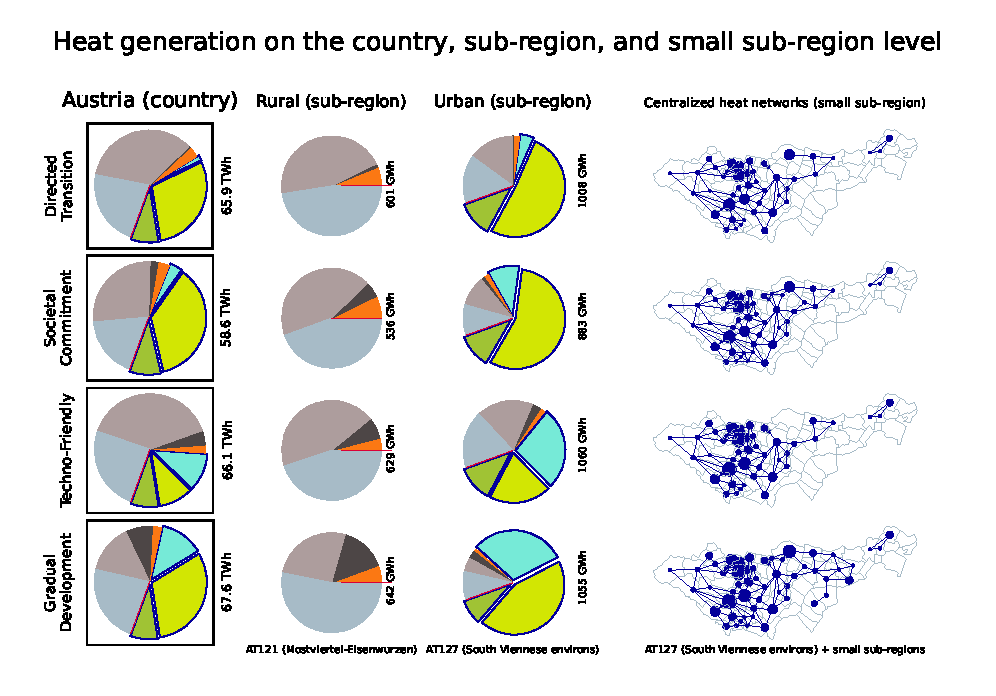
\includegraphics[width=1\linewidth]{figures/4_Results/Fig_Matrix-plot/Spatial_results.eps}
	\caption{Heat technology generation on different spatial granularity levels in the different scenarios supplying the residential and commercial heat demand. left: on the country level. middle: comparison of a rural and urban sub-region. right: centralized heat network topology (size of the points represent the amount of heat demand supplied by the network)}
	\label{fig:res1}
\end{sidewaysfigure}

\begin{figure}
	\centering
	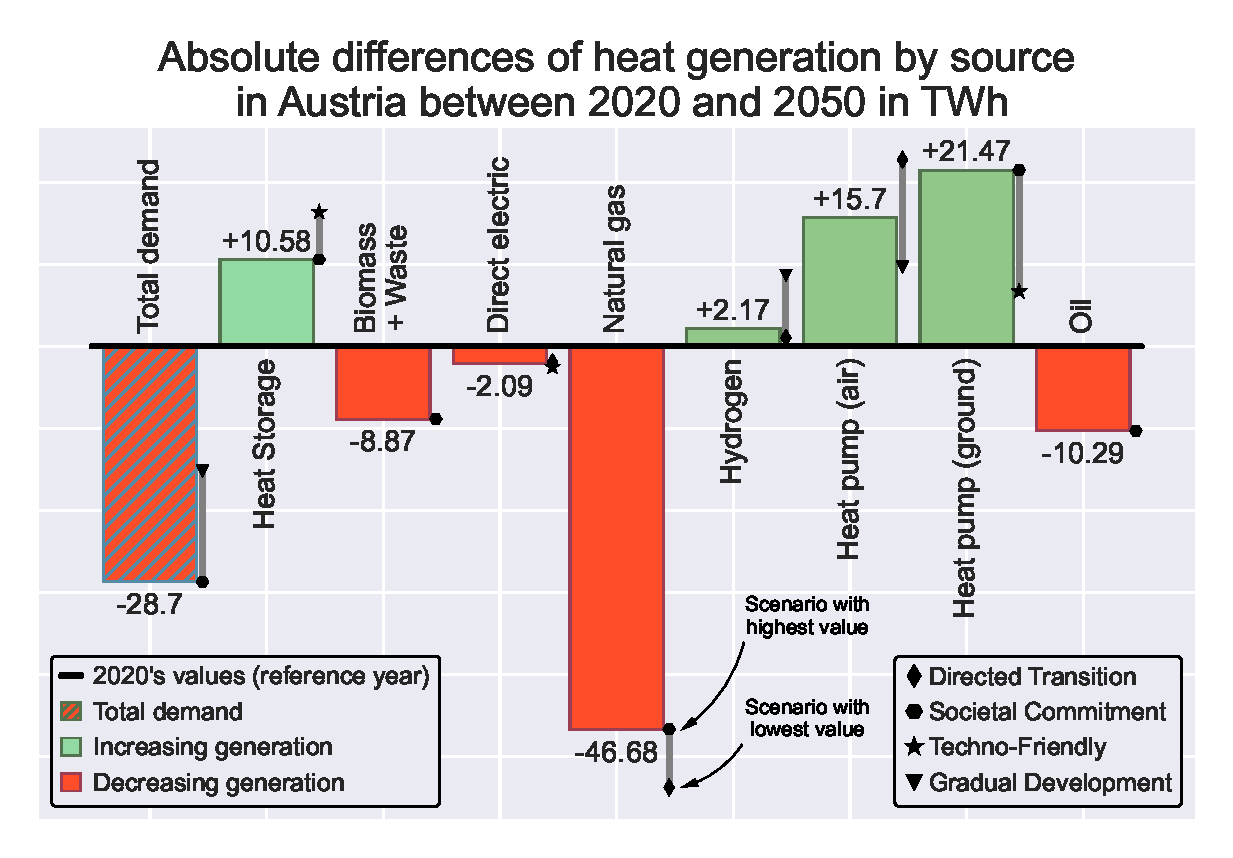
\includegraphics[width=1\linewidth]{figures/4_Results/Fig-Comp/Ref-2050.eps}
	\caption{Comparison of heat generation by source between the reference year $2020$ (black line) and 2050 in Austria. The height of the bars shows the absolute increase/decrease $2050$ in the \textit{Societal Commitment} scenario. The scenario with the lowest and highest difference, respectively, is indicated by the markers.}
	\label{fig:res-comp}
\end{figure}

\subsection{Sub-regions in Austria 2050 with high potentials for centralized heat supply}\label{res:3}
The potentials of centralized heat supply in Austria 2050 are limited to densely populated areas (urban areas). In particular, the results indicate only six different sub-regions (NUTS3 regions) that are supplied by centralized heat networks (see Figure \ref{fig:res2}). Although the exact numerical numbers differ, the six sub-regions in each scenario are (partially) supplied by centralized heat networks. Table \ref{tab:3} shows the centralized and on-site heat supply in the six sub-regions. Thereby, the connection rate is assessed by the share of centralized heat supply in the total heat demand. The population density varies in the six sub-regions between \SI{229}{persons \per \kilo\metre^2} (AT323 - Salzburg and sourroundings) and \SI{5124}{persons \per \kilo\metre^2} (AT130 - Vienna).

\begin{table} \centering
	\scalebox{1}{
		\renewcommand{\arraystretch}{1.35}
		\begin{tabular}{cccccc}
			\toprule 
			&& \multicolumn{2}{c}{in TWh} & in \%\\\cmidrule(lr){3-5}
			Sub-region & Storyline&Centralized & On-site & Connection rate\\\hline
			\parbox[t]{15mm}{\multirow{4}{*}{\rotatebox[origin=c]{90}{\parbox{2cm}{\centering South Viennesse\\environs (AT127)}}}} & Directed Transition & 0.72 & 0.17 & 81\\
			 & Societal Commitment & 0.78 & 0.11 & 88\\
			 & Techno-Friendly & 0.90 & 0.24 & 79\\
			 & Gradual Development & 1.20 & 0.09 & 93\\\hline
			 \parbox[t]{15mm}{\multirow{4}{*}{\rotatebox[origin=c]{90}{\parbox{2cm}{\centering Vienna\\(AT130)}}}} & Directed Transition & 3.98 & 0.95 & 81\\
			 & Societal Commitment & 4.28 & 0.61 & 88\\
			 & Techno-Friendly & 4.98 & 1.33 & 79\\
			 & Gradual Development & 6.59 & 0.47 & 93\\\hline
			  \parbox[t]{15mm}{\multirow{4}{*}{\rotatebox[origin=c]{90}{\parbox{2cm}{\centering Graz\\(AT221)}}}} & Directed Transition & 0.92 & 0.22 & 81\\
			 & Societal Commitment & 1.53 & 0.14 & 92\\
			 & Techno-Friendly & 1.16 & 0.31 & 79\\
			 & Gradual Development & 1.53 & 0.11 & 93\\\hline
			 \parbox[t]{15mm}{\multirow{4}{*}{\rotatebox[origin=c]{90}{\parbox{2cm}{\centering Linz-Wels\\(AT312)}}}} & Directed Transition & 1.24 & 0.30 & 81\\
			 & Societal Commitment & 1.34 & 0.19 & 88\\
			 & Techno-Friendly & 1.56 & 0.42 & 79\\
			 & Gradual Development & 2.06 & 0.15 & 93\\\hline
			  			\parbox[t]{15mm}{\multirow{4}{*}{\rotatebox[origin=c]{90}{\parbox{2cm}{\centering Salzburg and surroundings\\(AT323)}}}} & Directed Transition & 0.75 & 0.18 & 81\\
			 & Societal Commitment & 1.24 & 0.11 & 92\\
			 & Techno-Friendly & 0.93 & 0.25 & 79\\
			 & Gradual Development & 1.24 & 0.09 & 93\\\hline
			 \parbox[t]{15mm}{\multirow{4}{*}{\rotatebox[origin=c]{90}{\parbox{2cm}{\centering Rheintal-Bodensee\\(AT342)}}}} & Directed Transition & 0.66 & 0.16 & 81\\
			 & Societal Commitment & 0.71 & 0.10 & 88\\
			 & Techno-Friendly & 0.82 & 0.22 & 79\\
			 & Gradual Development & 1.09 & 0.08 & 93\\\hline
			 & & \multicolumn{2}{c}{Average connection rate}& \SI{85.25}{\%}\\
			\bottomrule
	\end{tabular}}
	\caption{Centralized heat supply and on-site heat generation in the six Austrian sub-regions, with potentials of centralized heat networks in 2050}
	\label{tab:3}
\end{table}

\begin{sidewaysfigure}
	\centering
	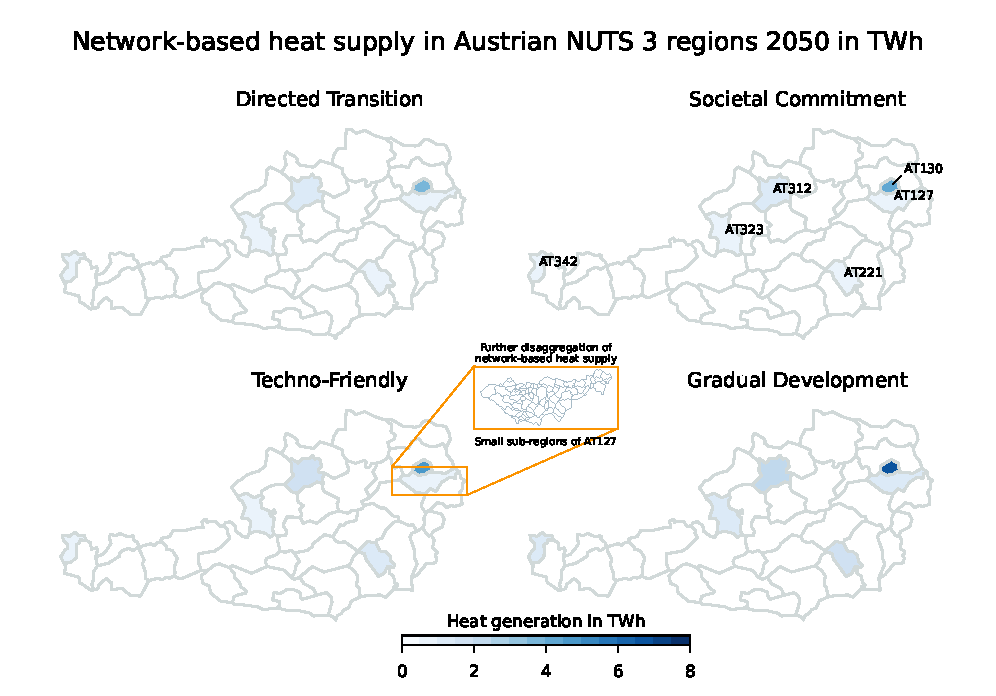
\includegraphics[width=1\linewidth]{figures/4_Results/Heatmap.eps}
	\caption{Centralized heat supply in Austria 2050}
	\label{fig:res2}
\end{sidewaysfigure}

\subsection{Centralized heat network topology on the community level}\label{res:4}
This section presents the centralized heat network topology of the sub-region \textit{South Viennese environs} (AT127) and all included communities. In Figure \ref{fig:res2}, this particular sub-region is marked by the orange box and figure \ref{fig:res3} shows the projected centralized heat network topology. In particular, the network topology is presented for the initial condition (as result of the sequential downscaling, $i=1$) and in the final condition ($i=29$) of the network. The distribution of the benchmark indicator values of the centralized heat network depending on the number of iterations is presented in the middle. Thereby, the mean value is marked in orange and increases with the number of iterations (increase from one third to almost two). Within the algorithm, this is achieved by reducing the supply area (decline in connected communities from 75 to 47). At the same time, the number of connected population decreases by \SI{13.3}{\%}, starting from a population of \SI{386}{k} being connected to centralized heating network in the before the first iteration. After the final iteration ($i=29$), the termination criterion is reached. A possible following step of iteration could not increase the benchmark indicator mean value any further. The iterative reduction of supplied small sub-regions does not necessarily result one contiguous graph. For example, three communities form a subgraph that is separate from the other network (see upper right in the final condition network graph). The results discussed above suggest that reducing the number of small sub-regions supplied by the centralized heat network increases the indicator value and thus the efficiency of the heat network topology. Simultaneously, this also increases the heat density of the supply area. In the following subsection, the obtained heat density values of the heat networks are compared with existing values and today's minimum required values for centralized heat networks.

\begin{sidewaysfigure}
	\centering
	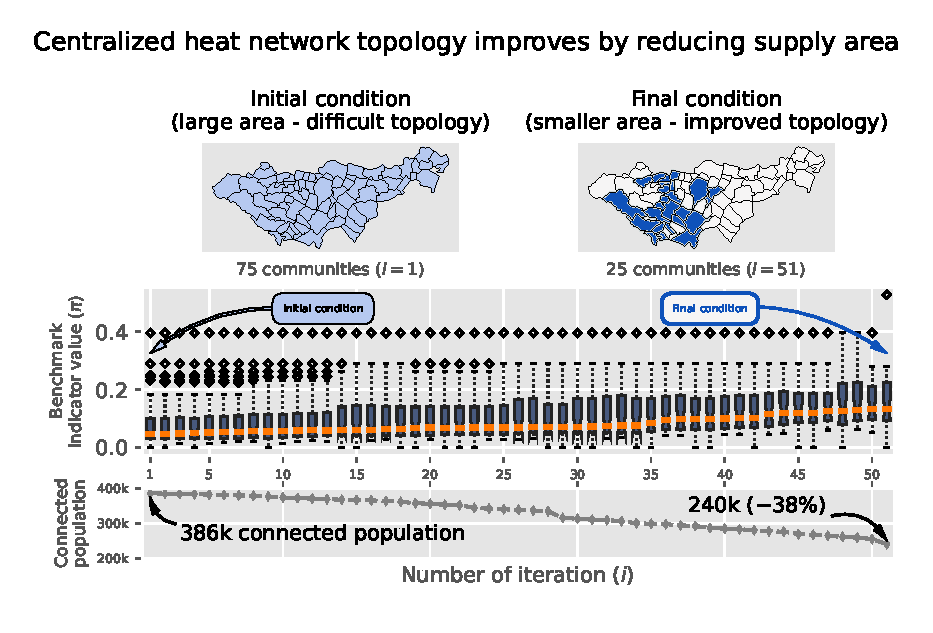
\includegraphics[width=1\linewidth]{figures/4_Results/Fig_Boxplot/ext_boxplot.eps}
	\caption{Centralized heat network topology in the initial and final condition. The boxplot (middle) indicates the improved network topology by an increasing benchmark indicator mean value (orange line). In the final condition, the connected population declines by \SI{-13.3}{\%} compared to the initial condition.}
	\label{fig:res3}
\end{sidewaysfigure}

\subsection{Comparison of 2050's and today's centralized heat networks using heat density as criterion}\label{res:5}
In the following, the centralized heat network in \textit{Graz} (AT221) is investigated in detail. Figure \ref{fig:res5} shows the heat density of the centralized heat network in the \textit{Techno-Friendly} scenario. The x-axis shows the three different downscaling techniques. The numerical numbers indicate an significant increase of the heat density resulting by the prioritized preference of heat sources (+\SI{1.07}{GWh \per km^2}) and the network topology benchmarking (+\SI{1.08}{GWh \per km^2}). However, comparing the obtained heat density value with heat density values of today's centralized heat networks reveals a signifcant gap (see the pink bar). According to references from the practice (see, e.g., in \url{http://www.austrian-heatmap.gv.at/ergebnisse/}), the heat density of today's networks is assumed to be \SI{10}{\frac{GWh}{km^2}} with a connection rate of \SI{90}{\%}. In general, the gap of heat density varies between the different scenarios. The smallest is achieved in the \textit{Techno-Friendly} scenario and amounts to \SI{7.42}{\frac{GWh}{km^2}} as presented in Figure \ref{fig:res5} by the pink bar. The largest gap is seen in the \textit{Societal Commitment} scenario and is \SI{8.41}{\frac{GWh}{km^2}}. The presented results of the sub-region are representative for the other sub-regions with potentials of centralized heat networks (excluding \textit{Vienna} (AT130)). Figure \ref{fig:res4} presents for the six different sub-regions the heat density values 2050 and the correspondig heat density gap. The heat density gap of \textit{Graz} in the \textit{Directed Transition} scenario is highlighted similar to the presentation in Figure \ref{fig:res5}. In particular, the results indicate no heat density gap for \textit{Vienna} (AT130) in all the scenarios, except a minor one in the results obtained using \textit{Directed Transition} scenario.  

\begin{figure}[h]
	\centering
	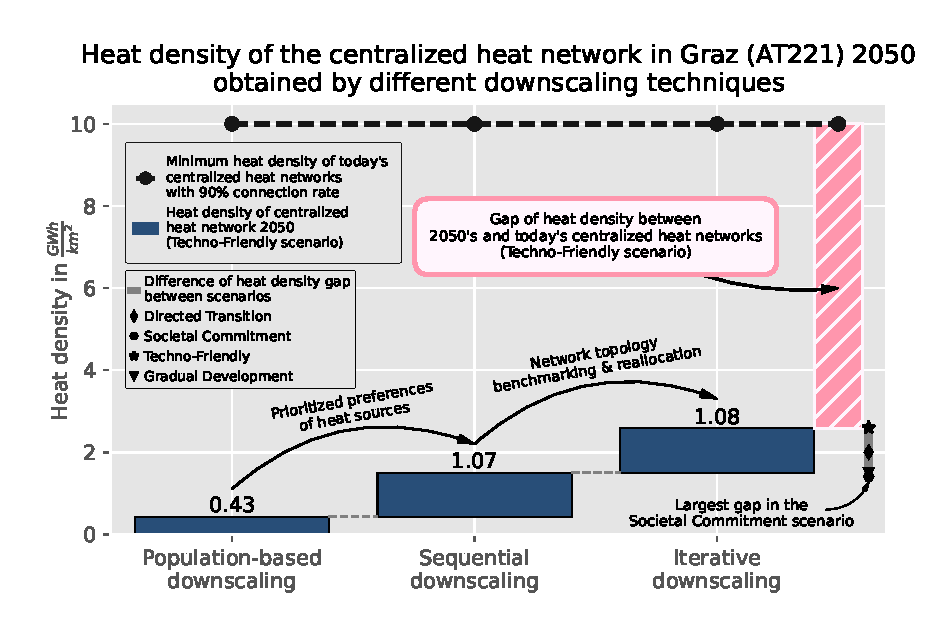
\includegraphics[width=1\linewidth]{figures/4_Results/Fig_Heat-density/HD_cleaned1.eps}
	\caption{Heat density of the centralized heat network in \textit{Graz} (AT221) 2050 in the \textit{Techno-Friendly} scenario. The gap of heat density between 2050's and today's heat density (black dashed line) is marked by the pink bar.}
	\label{fig:res5}
\end{figure}

\begin{figure}[h]
	\centering
	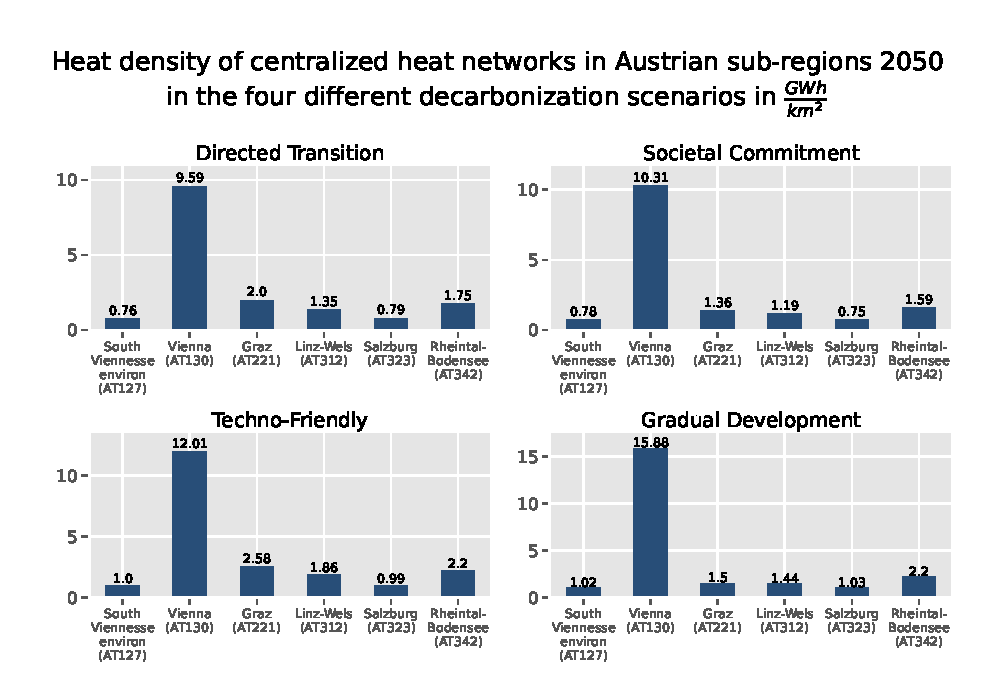
\includegraphics[width=1\linewidth]{figures/4_Results/Fig_Gap/HD1.eps}
	\caption{Heat densities (blue bars) of centralized heat networks in the six Austrian sub-regions and in the four different decarbonization scenarios. The heat density gap to today's centralized heat networks is indicated in pink. The smallest heat density gap (excluding \textit{Vienna} (AT130) is marked by the white hatch.)}
	\label{fig:res4}
\end{figure}
\newpage
\section{Conclusions and recommendations}\label{conclusions}
Sustainable energy transition requires methods to bridge the gap between global decarbonization plans and the resulting necessary measures at the local level. This work emphasizes the development of different downscaling algorithms in general, and the downscaling of the Austrian heating sector (residential and commercial) under the 1.5°C climate target to the community and grid levels in particular, considering technology-specific infrastructure requirements for the highly efficient usage of heat sources.\vspace{0.3cm}

We found that the prioritized perspective of efficiency and local utilization of renewable heat sources leads to a crucial treatment of the further development of district heating networks in the decarbonized Austrian heat supply toward 2050. This implies small-scale ($<\SI{1}{TWh}$) and large-scale ($>\SI{12}{TWh}$) district heating networks in terms of the amount of heat delivered. The results demonstrate that particularly densely populated areas are still beneficial supply areas for district heating networks and offer adequate heat densities. Nevertheless, most district heating networks in 2050 (seven of eight) will not reach the heat density benchmarks of today's networks and have a significant heat density gap. However, considering the increasing importance of local renewable heat sources feeding into district heating networks, we assume that these centralized networks will become required in the future and crucial in the decarbonization of the heating sector.\vspace{0.3cm}

We anticipate our work as a starting point, discussing the role of centralized heat networks as an infrastructure hub in the light of enabling large-scale, highly efficient, and local integration of renewable heat sources (such as biomass/waste, hydrogen, ground-sourced heat pumps, or geothermal units). In particular, we see a need for further research on the trade-off analysis between the efficiency/local integration of heat sources and the cost-intensive deployment of district heating networks. Future work may elaborate on the increasing cooling demand and how the cooperative design of district heating and cooling networks can contribute to the profitability of centralized heating and cooling infrastructure. 




\section*{Declaration of interests}
None.
\section*{Declaration of Competing Interest}
The authors report no declarations of interest.
\section*{Acknowledgments}
This project has received funding from the European Union's Horizon 2020 Research and Innovation Programme under Grant Agreement No. 835896. Part of the research was developed in the
Young Scientists Summer Program (YSSP) at the International Institute for Applied Systems Analysis(IIASA), Laxenburg (Austria).

\bibliography{mybibfile}
\appendix
\setcounter{table}{0}
\setcounter{figure}{0}


\section{Data and further empirical settings}\label{appendixA}
\begin{table}[h]
	\centering
	\scalebox{0.85}{
		\renewcommand{\arraystretch}{1.35}
		\begin{tabular}{lccc}
			\toprule 
			& Description & Data availability & Data source\\\hline
			GENeSYS-MOD v2.0 & Heat generation by source & \cite{explorer} & \cite{loffler2017designing}\\
			Austrian population density & in 2019 & \href{https://www.statistik.at/web_de/statistiken/index.html}{\textit{Statistik Austria}} & as availability\\
			Austrian population & in 2050 & \href{https://ec.europa.eu/eurostat/databrowser/view/tps00003/default/table?lang=en}{\textit{Eurostat}} & as availability\\
			\bottomrule
	\end{tabular}}
	\caption{Empirical data settings}
	\label{tab:a2}
\end{table}


\end{document}